\ChapterWithAuthor{Sume parțiale}{Andrei-Cristian Ivan}

\section{Problema inițială}

Să presupunem că avem un șir $V$ de $N$ numere indexat de la $1$, iar asupra șirului primim mai multe întrebări de forma: \emph{care este suma valorilor cuprinse între pozițiile $st$ și $dr$ (inclusiv) în șir?}

Răspunsul pentru această întrebare se poate calcula foarte ușor dacă realizăm parcurgerea efectivă a șirului de la poziția $st$ la poziția $dr$ și ne-ar lua \O{N} pași în cel mai rău caz ca să răspundem la o întrebare, complexitatea finală a programului ajungând la \O{N \cdot Q}, ceea ce pentru valori mai mari de $10^4$ pentru $N$ și $Q$ ar depăși limitele de timp la majoritatea problemelor de algoritmică. Așadar, este nevoie de o optimizare, care se numește \emph{„Sume parțiale”}.

\section{Prezentarea conceptului}

Sumele parțiale reprezintă o optimizare pentru algoritmii care trebuie să afle o sumă pe un interval, iar pe acel interval \textbf{nu} se produc modificări. Considerăm:

\begin{center}
    $sp[i] =$ suma valorilor de pe prefixul $1, 2, \dots, i$
\end{center}

Tabloul se calculează în felul următor:

\cpp{codes/sumepartiale/sp1.cpp}

După calculare, putem începe să răspunem la întrebări. Răspunsul nostru pentru un interval va fi:

\begin{center}
    $suma \ = sp[dr] - sp[st - 1]$
\end{center}

Faptul că răspunsul nostru este dat de o formulă, va face ca timpul nostru efectuat pentru rezolvarea unei întrebări să fie constant \O{1}, ceea ce va duce ca programul nostru să aibă o complexitate finală \O{N + Q}, pentru calcularea tabloului $sp$ și pentru citirea și răspunderea la întrebări. Totuși, hai să vedem de formula menționată mai sus funcționează. 

Pentru demonstrație, vom încerca o abordare grafică a formulei. Primul pas constă în adunarea sumei prefixului $1, 2, \dots, dr$.

\begin{center}
    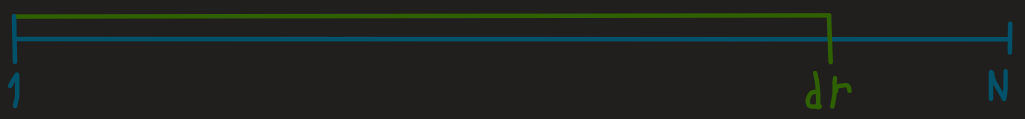
\includegraphics[width=\textwidth]{images/sumepartiale/sp1.png}
\end{center}

Apoi, va trebui să scădem prefixul $1, 2, \dots, st - 1$.

\begin{center}
    
\includegraphics[width=\textwidth]{images/sumepartiale/sp2.png}
\end{center}

În final, subsecvența $st, st + 1, \dots, dr - 1, dr$ va fi alcătuită din acele poziții care se află în segmentul \emph{verde} (prefixul $1, 2, \dots, dr$), dar care nu se află și în segmentul \emph{roșu} (prefixul $1, 2, \dots, st - 1$). Așadar, în urma acestei delimitări o să obținem suma cerută pe intervalul nostru.

\section{Extinderea sumelor parțiale pe matrice}

\section{Șmenul lui \emph{Mars} (1D/2D)}